\section {Comparison to other DVCS}\label{comparisontootherdvcs}

There are several more distributed version control systems.
We are going to explain some differences to Git.
Some are:

  \begin{enumerate}
     \item \emph{Bazaar}. Powered by Cannocial. Handles the whole Ubuntu source
     repository at launchpad.net
     \item \emph{Mercurial} An opensource project initiated by Matt Mackall
     \item \emph{Perforce}. Powered by Perforce Software Inc.
     \item \emph{Visual SourceSafe} Powered by Microsoft
  \end{enumerate}
  
We are going to take a closer look at \emph{Baazar} and \emph{Mercurial} 
compared to Git.

\subsection {Data storage}

As already mentioned Git uses its unique storage model creating new snapshots
every commit. Mercurial also thinks of its data as a snapshot. The difference
is though, that basically Mercurial also creates deltas from a revision A to B.
Those deltas are in fact the difference between two revisions. When a cumulative
amount of deltas is stored to a file, Mercurial creates a new snapshot of this file. 
\cite[chapter 4]{hgbook2009} 

Baazar plans to change its model and uses socalled \emph{nested trees}. At the level of data storage they are quite similar to Git. The difference is that nested trees use unversioned branch data to store data instead of version files. \footnote{ http://wiki.bazaar.canonical.com/NestedTreesDesign\#git-submodules on 21.11.2010 } Baazar is not well documented. In fact there are very good tutorials on how to use Baazar, but when it comes to technical details, there is not much official documentation.

\subsection {Speed and size}

Git claims to be a very efficient system. To measure that there are several
methods. The website \emph{whygitisbetterthanx.com} did a quite good job to
summarize why Git does handle things quite fast.
Some of these tests are very biased and it seems obvious that the author's favourite system is Git. 
But there are three tests\footnote{http://doc.bazaar.canonical.com/migration/en/why-switch-to-bazaar.html\#high-storage-efficiency-and-speed on 21.11.2010} on the Baazar homepage that show that Git clearly wins 
calculating the differences from revision A to B, commiting and using the log command:

\begin{figure}[h]
  \centering
  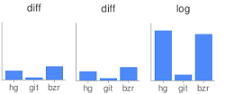
\includegraphics{img/speed.png}
  \caption{Speed tests}
  \label{fig:Speedtests}  
\end{figure}

The measured time\footnote{http://doc.bazaar.canonical.com/migration/en/why-switch-to-bazaar.html\#high-storage-efficiency-and-speed on 21.11.2010} can be seen in table \ref{tab:time}\\

\begin{tabular}{ l || l | l | l }
Operation &	Mercurial &	Git & Bazaar \\
\hline
diff & 0.622s & 0.156s & 0.916s\\
commit & 1.126s & 0.348s & 1.030s\\
log & 3.449s & 0.402s & 3.205s\\
\label{tab:time}
\end{tabular}\\

Considering the size of the metadata including the content created by the DVCS there are other several tests. Here is another test from the Baazar homepage:

Figure \ref{fig:mozilla} shows how much space the imported Mozilla project Firefox 3.5 has in the three different version control systems. Table \ref{tab:mozilla} lists how much MB each of them needed.

\begin{figure}[h]
  \centering
  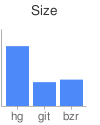
\includegraphics{img/size.png}
  \caption{Size of imported Mozilla project}
  \label{fig:mozilla}  
\end{figure}

\begin{center}
\begin{tabular}{ l | c | r }
Mercurial &	Git & Bazaar \\
\hline
311M & 124M & 137M
\end{tabular}
\label{tab:mozilla}
\end{center}


